\documentclass[14pt]{extbook}
\usepackage{multicol, enumerate, enumitem, hyperref, color, soul, setspace, parskip, fancyhdr} %General Packages
\usepackage{amssymb, amsthm, amsmath, latexsym, units, mathtools} %Math Packages
\everymath{\displaystyle} %All math in Display Style
% Packages with additional options
\usepackage[headsep=0.5cm,headheight=12pt, left=1 in,right= 1 in,top= 1 in,bottom= 1 in]{geometry}
\usepackage[usenames,dvipsnames]{xcolor}
\usepackage{dashrule}  % Package to use the command below to create lines between items
\newcommand{\litem}[1]{\item#1\hspace*{-1cm}\rule{\textwidth}{0.4pt}}
\pagestyle{fancy}
\lhead{Progress Quiz 8}
\chead{}
\rhead{Version A}
\lfoot{5493-4176}
\cfoot{}
\rfoot{Summer C 2021}
\begin{document}

\begin{enumerate}
\litem{
Determine the horizontal and/or oblique asymptotes in the rational function below.\[ f(x) = \frac{6x^{3} +29 x^{2} -5 x -100}{3x^{2} +10 x -25} \]\begin{enumerate}[label=\Alph*.]
\item \( \text{Horizontal Asymptote of } y = 2.0  \)
\item \( \text{Horizontal Asymptote of } y = 2.0 \text{ and Oblique Asymptote of } y = 2x + 3 \)
\item \( \text{Oblique Asymptote of } y = 2x + 3. \)
\item \( \text{Horizontal Asymptote of } y = -5.0 \text{ and Oblique Asymptote of } y = 2x + 3 \)
\item \( \text{Horizontal Asymptote at } y = -5.0 \)

\end{enumerate} }
\litem{
Determine the vertical asymptotes and holes in the rational function below.\[ f(x) = \frac{16x^{3} +64 x^{2} +79 x + 30}{12x^{2} +x -6} \]\begin{enumerate}[label=\Alph*.]
\item \( \text{Vertical Asymptote of } x = 0.667 \text{ and hole at } x = -0.75 \)
\item \( \text{Holes at } x = 0.667 \text{ and } x = -0.75 \text{ with no vertical asymptotes.} \)
\item \( \text{Vertical Asymptotes of } x = 0.667 \text{ and } x = -0.75 \text{ with no holes.} \)
\item \( \text{Vertical Asymptote of } x = 1.333 \text{ and hole at } x = -0.75 \)
\item \( \text{Vertical Asymptotes of } x = 0.667 \text{ and } x = -1.25 \text{ with a hole at } x = -0.75 \)

\end{enumerate} }
\litem{
Determine the horizontal and/or oblique asymptotes in the rational function below.\[ f(x) = \frac{3x^{2} -7 x -20}{9x^{3} +18 x^{2} -7 x -20} \]\begin{enumerate}[label=\Alph*.]
\item \( \text{Horizontal Asymptote of } y = 0 \)
\item \( \text{Horizontal Asymptote of } y = 0.333  \)
\item \( \text{Horizontal Asymptote at } y = 4.000 \)
\item \( \text{Horizontal Asymptote of } y = 0.333 \text{ and Oblique Asymptote of } y = 3x + 13 \)
\item \( \text{Oblique Asymptote of } y = 3x + 13. \)

\end{enumerate} }
\litem{
Which of the following functions \textit{could} be the graph below?
\begin{center}
    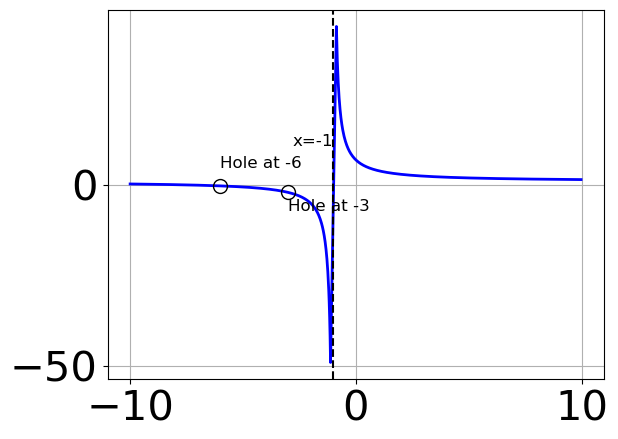
\includegraphics[width=0.5\textwidth]{../Figures/identifyGraphOfRationalFunctionA.png}
\end{center}
\begin{enumerate}[label=\Alph*.]
\item \( f(x)=\frac{x^{3} +3.0 x^{2} -40.0 x -84.0}{x^{3} +10.0 x^{2} +27.0 x + 18.0} \)
\item \( f(x)=\frac{x^{3} -16.0 x^{2} +81.0 x -126.0}{x^{3} -10.0 x^{2} +27.0 x -18.0} \)
\item \( f(x)=\frac{x^{3} + x^{2} -44.0 x -84.0}{x^{3} -10.0 x^{2} +27.0 x -18.0} \)
\item \( f(x)=\frac{x^{3} +16.0 x^{2} +81.0 x + 126.0}{x^{3} +10.0 x^{2} +27.0 x + 18.0} \)
\item \( \text{None of the above are possible equations for the graph.} \)

\end{enumerate} }
\litem{
Determine the vertical asymptotes and holes in the rational function below.\[ f(x) = \frac{6x^{3} +11 x^{2} -5 x -12}{12x^{2} +25 x + 12} \]\begin{enumerate}[label=\Alph*.]
\item \( \text{Vertical Asymptotes of } x = -0.75 \text{ and } x = -1.5 \text{ with a hole at } x = -1.333 \)
\item \( \text{Vertical Asymptotes of } x = -0.75 \text{ and } x = -1.333 \text{ with no holes.} \)
\item \( \text{Vertical Asymptote of } x = 0.5 \text{ and hole at } x = -1.333 \)
\item \( \text{Vertical Asymptote of } x = -0.75 \text{ and hole at } x = -1.333 \)
\item \( \text{Holes at } x = -0.75 \text{ and } x = -1.333 \text{ with no vertical asymptotes.} \)

\end{enumerate} }
\litem{
Determine the horizontal and/or oblique asymptotes in the rational function below.\[ f(x) = \frac{6x^{3} +13 x^{2} -13 x -30}{2x^{2} +3 x -9} \]\begin{enumerate}[label=\Alph*.]
\item \( \text{Horizontal Asymptote of } y = -3.0 \text{ and Oblique Asymptote of } y = 3x + 2 \)
\item \( \text{Oblique Asymptote of } y = 3x + 2. \)
\item \( \text{Horizontal Asymptote of } y = 3.0  \)
\item \( \text{Horizontal Asymptote of } y = 3.0 \text{ and Oblique Asymptote of } y = 3x + 2 \)
\item \( \text{Horizontal Asymptote at } y = -3.0 \)

\end{enumerate} }
\litem{
Determine the horizontal and/or oblique asymptotes in the rational function below.\[ f(x) = \frac{6x^{2} +29 x + 20}{12x^{3} +76 x^{2} +145 x + 75} \]\begin{enumerate}[label=\Alph*.]
\item \( \text{Horizontal Asymptote of } y = 0.500  \)
\item \( \text{Oblique Asymptote of } y = 2x + 3. \)
\item \( \text{Horizontal Asymptote of } y = 0 \)
\item \( \text{Horizontal Asymptote of } y = 0.500 \text{ and Oblique Asymptote of } y = 2x + 3 \)
\item \( \text{Horizontal Asymptote at } y = -4.000 \)

\end{enumerate} }
\litem{
Which of the following functions \textit{could} be the graph below?
\begin{center}
    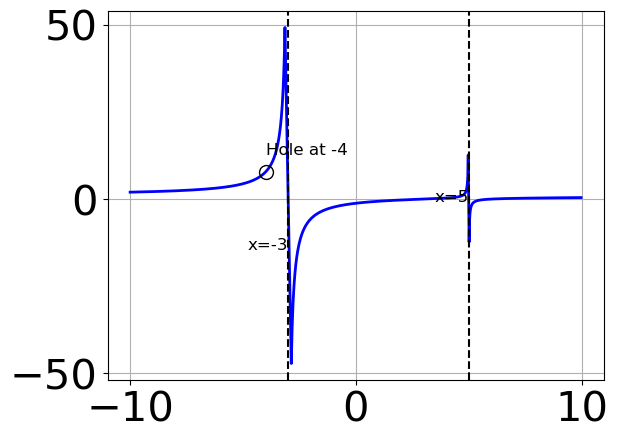
\includegraphics[width=0.5\textwidth]{../Figures/identifyGraphOfRationalFunctionCopyA.png}
\end{center}
\begin{enumerate}[label=\Alph*.]
\item \( f(x)=\frac{x^{3} +5.0 x^{2} -18.0 x -72.0}{x^{3} -2.0 x^{2} -23.0 x + 60.0} \)
\item \( f(x)=\frac{x^{3} -5.0 x^{2} -18.0 x + 72.0}{x^{3} +2.0 x^{2} -23.0 x -60.0} \)
\item \( f(x)=\frac{x^{3} +12.0 x^{2} +45.0 x + 54.0}{x^{3} -2.0 x^{2} -23.0 x + 60.0} \)
\item \( f(x)=\frac{x^{3} -2.0 x^{2} -45.0 x + 126.0}{x^{3} +2.0 x^{2} -23.0 x -60.0} \)
\item \( \text{None of the above are possible equations for the graph.} \)

\end{enumerate} }
\litem{
Determine the vertical asymptotes and holes in the rational function below.\[ f(x) = \frac{9x^{3} -28 x -16}{9x^{2} +6 x -8} \]\begin{enumerate}[label=\Alph*.]
\item \( \text{Vertical Asymptote of } x = 1.0 \text{ and hole at } x = -1.333 \)
\item \( \text{Vertical Asymptote of } x = 0.667 \text{ and hole at } x = -1.333 \)
\item \( \text{Vertical Asymptotes of } x = 0.667 \text{ and } x = -0.667 \text{ with a hole at } x = -1.333 \)
\item \( \text{Holes at } x = 0.667 \text{ and } x = -1.333 \text{ with no vertical asymptotes.} \)
\item \( \text{Vertical Asymptotes of } x = 0.667 \text{ and } x = -1.333 \text{ with no holes.} \)

\end{enumerate} }
\litem{
Determine the vertical asymptotes and holes in the rational function below.\[ f(x) = \frac{12x^{3} +53 x^{2} +73 x + 30}{12x^{2} +x -6} \]\begin{enumerate}[label=\Alph*.]
\item \( \text{Vertical Asymptotes of } x = 0.667 \text{ and } x = -1.667 \text{ with a hole at } x = -0.75 \)
\item \( \text{Vertical Asymptotes of } x = 0.667 \text{ and } x = -0.75 \text{ with no holes.} \)
\item \( \text{Vertical Asymptote of } x = 0.667 \text{ and hole at } x = -0.75 \)
\item \( \text{Holes at } x = 0.667 \text{ and } x = -0.75 \text{ with no vertical asymptotes.} \)
\item \( \text{Vertical Asymptote of } x = 1.0 \text{ and hole at } x = -0.75 \)

\end{enumerate} }
\end{enumerate}

\end{document}